\documentclass[11pt]{article}
\usepackage[margin=1in]{geometry}
\usepackage[T1]{fontenc}
\usepackage{lmodern}
\usepackage{microtype}
\usepackage{amsmath,amssymb}
\usepackage{booktabs}
\usepackage{tabularx}
\newcolumntype{L}{>{\raggedright\arraybackslash}X}
\usepackage{graphicx}
\usepackage{xcolor}
\usepackage[numbers,sort&compress]{natbib}
\usepackage[hidelinks]{hyperref}
\usepackage{enumitem}
\setlist{nosep,leftmargin=1.4em}

% Numbers that are filled in as runs complete. Every number in the paper is traceable to a run
% folder under runs/ and to docs/IMPLEMENTATION.md, section 6.
\newcommand{\ie}{iE}

\title{What Limits a Five-Minute Coding Agent?\\Preference Directions, Query-Only Control,\\and the Cost of Terse Problem Statements}
\author{Tian Qin\\\small Google -- The Gemma 4 Developer Agent Paper Track}
\date{}

\begin{document}
\maketitle

\begin{abstract}
We study how far a fixed, 4-bit quantization-aware-trained Gemma~4 31B can be improved as a repository-level coding agent when only its declarative configuration and LoRA adapters may change and every task must finish in five minutes. The resolution rate is too noisy to steer by: two draws of one agent differ on 11 of 100 tasks. We therefore steer by a \emph{behaviour vector} of low-noise coordinates (malformed tool calls, repeat loops, time to the first edit, edit and empty-patch rates) on a budget calibrated to the scoring hardware. The diagnosis is one trade-off: with less thinking the model acts sooner but writes malformed tool calls. A \emph{format direction}, a rank-16 LoRA trained with NLL-anchored DPO on preference pairs mined at the agent's own failure states and rendered token-identically to the server, cuts malformed calls from 4--6\% to 0.3--0.6\% and loops from 10--13\% to 1--2\% on 100 tasks, replicated against two base draws; its resolution gain (+3.5 points) is within noise, and a seven-point gain that looked replicated vanished when the control was drawn again. We then use iterative Expectation (iE), an accelerated Robbins--Monro scheme from statistical bias reduction, as a query-only controller over sampling knobs and over exact merges of trained directions: the direction basis is well conditioned (condition number 5.6 against 591 for the knobs) and a direction compensates a harmful knob, but no controlled point beat the single direction. Finally we locate the gap between local scores (31--38\%) and the leaderboard's 13\%: not the scoring environment, repository familiarity or fix size, but the problem statement. Cutting statements to their titles reproduces the leaderboard's level (37\% to 17\%, $p = 0.0001$). On that proxy, better tools, guidance, speed, two forms of statement distillation and an iE calibration of a distilled direction's weight each change behaviour but not score: under a five-minute budget the binding constraint is the model's reasoning about an underspecified task.
\end{abstract}

\section{Introduction}

A competition harness that freezes the model, the tools and the time budget leaves a narrow space for improvement: prompts, sampling and budget settings, an agent hierarchy, and low-rank adapters. Inside that space the obvious objective, the fraction of tasks resolved, is a poor guide. Twenty-four tasks give a binomial standard deviation of two tasks; a hundred tasks still flip by a dozen between repeated draws of the same agent. Prompt and sampling variants routinely land within that noise of each other, so a search driven by the score mostly chases noise, and, as our own results show, even a difference that replicates in one arm of a comparison can be an artifact of a single draw of the other.

This paper reports a different route, taken end to end on one model and one harness (the Gemma~4 Developer Agent competition; Section~\ref{sec:setting}). We make four contributions.

\begin{enumerate}
  \item \textbf{Measurement before tuning.} We calibrate the local budget to the scoring hardware by per-turn timing, establish a repeated-draw noise floor, and steer by a vector of behaviour coordinates whose run-to-run spread is far smaller than the score's (Section~\ref{sec:measure}). The vector exposes the failure that matters: a thinking budget trades decisiveness against well-formed tool calls (Section~\ref{sec:diagnosis}).
  \item \textbf{On-policy preference directions.} We build LoRA adapters from preference pairs mined at the agent's own failure states, rendered exactly as the harness renders them and labelled by the harness's own matcher (Section~\ref{sec:directions}). The \emph{format direction} removes most malformed calls and loops on 100 public tasks, replicated against two draws of the base agent; its effect on resolution (+3.5 points pooled) is within the run-to-run noise we measure at that scale (Section~\ref{sec:results-format}). We document a collapse mode of whole-sequence DPO on near-identical pairs and the gate that prevents it.
  \item \textbf{Query-only control of directions.} We cast the remaining configuration space as a root-finding problem on the expected behaviour vector and solve it with iterative Expectation (iE)~\citep{qin2025ie}, using exact rank-stacked merges of trained adapters as the control (Section~\ref{sec:control}). The results are mixed and, we think, instructive: the direction basis is well conditioned where sampling knobs are not, and a direction compensates a harmful knob, but without a noise-aware merit gate and attainable targets the controller runs to its bounds, and in our runs the single format direction remained the best operating point (Section~\ref{sec:results-control}). In its original form, a moment equation solved by simulation, iE also calibrates a distilled direction cheaply at fixed agent states and shows when no weight can reach a per-call target; validated against our agent runs, the same fixed-state check does not predict effects that act through the trajectory (Section~\ref{sec:scaffold}). Making the informed agent's measured behaviour the target shows that more than half of the distance to it lies outside the directions' span.
  \item \textbf{Locating the leaderboard gap.} With a calibration run on the scoring hardware and two held-out task sets mined from recent commits of less-known repositories, we show that problem-statement informativeness, not repository familiarity, fix size or the scoring environment, accounts for most of the drop from local to leaderboard scores; an iE calibration over the fraction of the statement kept finds no fraction that reproduces the leaderboard's level, title-only being the nearest within noise; and we use the resulting leaderboard-matched proxy to test three scaffold changes and two forms of statement distillation (Sections~\ref{sec:gap} and~\ref{sec:scaffold}).
\end{enumerate}

\section{Setting}\label{sec:setting}

\paragraph{Model, harness and submission.} The model is \texttt{gemma-4-31b-it-qat-w4a16-ct}: Gemma~4 31B with 4-bit, group-32 integer weights from quantization-aware training, served by vLLM~\citep{kwon2023vllm} 0.19.1 with a competition patch for Gemma~4 LoRA, tensor-parallel over four NVIDIA L4 GPUs, with a 32,768-token context. A submission is a declarative bundle (Google ADK agent configuration, prompts, sampling settings, up to eight PEFT LoRA adapters of rank at most 128, under 3\,GiB); no submitted Python runs outside the task sandbox. Each task is a repository snapshot and a pull-request title and description, often a single line. The agent has shell, file read, file edit, file write and three code-graph tools; the harness grades the working-tree diff against hidden tests, even when the agent never calls \texttt{submit\_patch}. Conversation history is compacted by ADK once it passes 14,336 tokens. Midway through the competition the organisers also allowed three smaller Gemma~4 models (12B, E4B, E2B); we test the 12B in Section~\ref{sec:gap}.

\paragraph{Budget.} All roughly 120 hidden tasks run sequentially within 12 hours including server start-up, about six minutes per task on average. We cap each task at five minutes, which is safe in the worst case. That frame is our choice and not the competition's: the most-run public configuration~\citep{henao2026budgetfit} sets eight minutes bounded by 28 tool calls and fits the limit because most tasks finish early. We measured the scoring hardware with a private notebook: decode at 37 tokens/s (33 through a LoRA route), one agent turn at $0.46\,\text{s} + n_\text{tok}/31$, against $1.09\,\text{s} + n_\text{tok}/9.5$ on our local machine (an NVIDIA GB10 with unified memory). Every local run therefore uses a cap that buys the same token budget as five minutes on the scorer: 34 minutes at eight concurrent tasks. Our first comparisons, made before this calibration, ran at about a third of the real budget and reached conclusions that did not survive it, which is the main reason we report it.

\paragraph{Tasks.} The public set has 129 tasks from four repositories. We kept the 100 that grade soundly in our environment (every task fails with an empty patch and passes with its reference patch): 60 from \texttt{fastapi} and 40 from \texttt{rich}. A fixed random subset of 24 (12 from each) is used for quick comparisons (\emph{dev24}). The hidden set comes from private repositories, so absolute local numbers overstate the hidden-set score.

\section{Measuring under a tight budget}\label{sec:measure}

\paragraph{The behaviour vector.} For a run we compute, per call or per task: the malformed-call rate (argument keys that are not identifiers, a path that swallowed the next argument, or a harness reply that a mandatory argument is missing), the fraction of tasks with four or more identical consecutive calls (\emph{loops}), the median time to the first \texttt{edit\_file} in scorer-equivalent seconds, the fractions of patches that touch real source, that are empty, and that edit source but fail the tests (\emph{wrong edits}), and the number of context compactions per task. Rates are transformed to the logit scale and times to the log scale for control. Resolution is tracked in every run but never controlled.

\paragraph{Noise floor.} The same agent on dev24, twice: resolution 10 and 9 of 24, malformed calls 2.0\% and 2.9\%, first edit at 297 and 342 seconds, compactions 1.04 and 1.00 per task. On 100 tasks, two draws of the unmodified agent at identical settings resolved 31 and 38, agreeing on 29 resolved tasks and differing on 11; two draws of the format direction agreed on 32 and differed on 12. All comparisons below are against these spreads, and all claims about resolution are paired comparisons on identical task sets.

\paragraph{Selection bias.} Reporting the best of several configurations evaluated on the same tasks inflates the winner's rate, and several comparisons below are of that kind. We remove the bias with iE in its original role, the analytic iteration $x_{k+1} = x_k + (\alpha - M(x_k))$ with $M$ computed by simulation~\citep[Section~3.3]{qin2025ie}: the parameter $x$ is the vector of the $K$ configurations' true rates ordered by observed rank, the statistic $\alpha$ is the vector of observed pooled rates sorted ascending, and $M$ is the expectation of that sorted vector under a two-way logistic model, $\operatorname{logit} P(\text{resolved}) = a_i + b_j$ for task $i$ and configuration $j$, with $a_i \sim N(0, \tau^2)$ integrated out by quadrature (a point fit with one to thirteen outcomes per task makes every task deterministic) and each replicate drawing the fixed tasks' difficulties from their posteriors. The iterate is kept sorted, so tied observations stop the iteration at the boundary. The model is not fitted to the draw-to-draw disagreement and reproduces it: 11.1 tasks expected to differ between two base draws on the public set against 11 observed, 3.9 against 3 on dev24. Three results. On the 100 public tasks the format direction's advantage over the base is unchanged by de-biasing, $+3.5$ tasks against the base alone and $+4.1$ with the gated end point included, with a model standard deviation of 2.4 tasks; two arms separated by 3.5 tasks leave the maximum unbiased to a tenth of a task, and the winner's curse for the best of three at this noise is 1.6 tasks. On the 76 title-only hard tasks (Section~\ref{sec:scaffold}) the six configurations' observed spread, five at 13 and one at 4, is below what noise alone would produce: if all six had the base's rate the best would read 15.4 on average (standard deviation 1.5), so the equation has no root with distinct rates and no change is above the base. On dev24 the seven configurations compared at the calibrated budget pool to one de-biased rate of 8.8 of 24 (observed 7.5 to 9.5; the best of seven equal configurations would read 10.2), which is the quantitative form of ``within noise''.

\paragraph{Guarded evaluation.} Two infrastructure failures cost us full nights before we built a guard, and both would silently corrupt any comparison. At eight concurrent tasks, unlimited sandboxes starved the model server (aggregate decoding fell from about 40 to 2--9 tokens/s for ten hours); and a single agent-launched process grew to 42\,GB and took the whole evaluator down with it. Every run reported here therefore executes each sandbox command in its own control group with the scorer's sandbox limits (4\,GiB, two cores), with the evaluator at lower priority than the server and a watchdog that aborts a run whose server throughput collapses.

\section{Diagnosis: thinking trades decisiveness for well-formed calls}\label{sec:diagnosis}

Prompt changes altered what the model avoided (for example, it stopped writing reproduction scripts when asked) but not how decisively it acted. Sweeping the thinking budget did (Figure~\ref{fig:thinking}). With 512 or 128 tokens of thinking per turn, calls are almost always well formed, but the agent explores in small steps and rarely reaches an edit; with thinking off it edits in more than half of the tasks, but a quarter of its calls are malformed. The malformed calls have two signatures: a multi-line \texttt{edit\_file} whose string argument swallows the next argument, and a \texttt{read\_file} whose key is written in JSON style (\texttt{end\_line"}), so the range is silently ignored. Both arise deep in sessions, after many tool results that reach the model as JSON-escaped strings, while a clean single turn produces well-formed calls. At the calibrated budget the thinking-on agent does reach its edits (Section~\ref{sec:results-format}), and the malformed calls (4.2\% of all calls on 100 tasks) and loops (10\% of tasks) become the clearest remaining waste, which is what the first direction targets.

\begin{figure}[t]
  \centering
  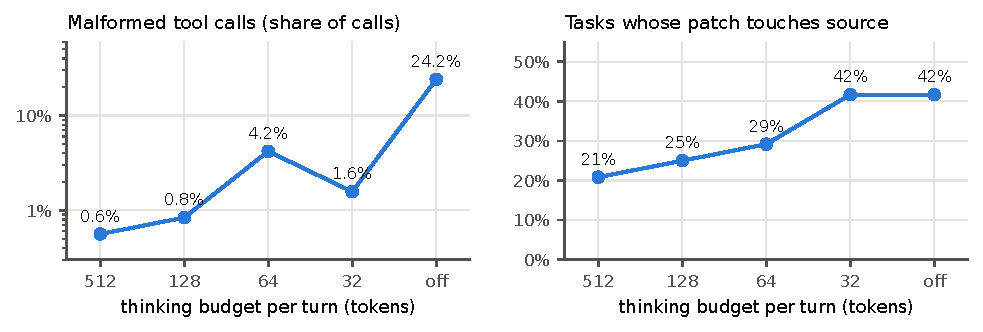
\includegraphics[width=\linewidth]{figures/thinking_tradeoff.pdf}
  \caption{Thinking budget against malformed tool calls and decisiveness, on dev24 with the same prompt (512: one task at a time with a five-minute cap; others: four requests in parallel with the cap scaled to the same token budget; both about a third of the calibrated budget). Left: malformed-call rate (log scale). Right: fraction of tasks whose patch touches real source.}
  \label{fig:thinking}
\end{figure}

\section{On-policy preference directions}\label{sec:directions}

A \emph{direction} is a rank-16 LoRA adapter on all seven projections of the 60 language-model layers (122M parameters), trained with DPO~\citep{rafailov2023dpo} on preference pairs that target one behaviour coordinate.

\subsection{Mining pairs where the agent fails}\label{sec:mining}

\paragraph{Exact context reconstruction.} Traces keep only parsed tool arguments, so the raw text of a malformed call is lost. We instead rebuild the context the model saw at every turn where it produced one, and sample new completions there. Matching the harness exactly required details that are documented nowhere: ADK appends an identity line to the system instruction; tool declarations come from the harness's Python signatures through ADK's conversion; tool results enter as \texttt{tool} messages carrying the JSON observation; and the thinking budget is not passed by ADK at all but bridged by the submission compiler into the request's chat-template arguments, so thinking on and off render different prompts. Each rebuilt context is checked against the trace's recorded prompt length, and for training we render with the tokenizer in a form verified to be token-for-token identical to the server's (Appendix~\ref{app:rendering}). Only turns before the first context compaction are used.

\paragraph{Labelling.} At each context we sample eight raw completions with special tokens kept and label each with a strict parser of the model's native call syntax (bare keys, strings delimited by a dedicated token); \texttt{edit\_file} calls are additionally run through the harness's own tiered matcher against the file state reconstructed at that step. A pair is a well-formed and a malformed call of the same tool from the same prefix. Where no well-formed call of that tool was sampled, the malformed one is repaired by its single format error and re-verified (55 of 148 contexts). From the three thinking-off development runs this yields 738 pairs from 148 contexts (289 \texttt{edit\_file}, 449 \texttt{read\_file}).

\subsection{Training on quantized weights}\label{sec:training}

The served checkpoint is decompressed to bf16 for training; integer group dequantization is exact, so the adapter is trained on the values the server computes with. Prefixes (up to 14k tokens) are truncated to 4,096 tokens for training, keeping the first 512 (system prompt and task) and the most recent 3,584. Each prefix is run once without gradient and its key--value cache kept; chosen and rejected completions are scored against the cache with the adapter, and reference log-probabilities come from the same model with the adapter disabled. Gradient therefore flows only through the completion tokens, which is the behaviour the direction is about, and long contexts stay affordable. On this GPU attention scores are materialized, so a full completion graph does not fit beside the 60\,GiB model at long prefixes; we compute the DPO margin without gradient and back-propagate each completion separately, in 96-token chunks with the cache detached between chunks (Appendix~\ref{app:training}). Peak memory is 81\,GiB at a 4k-token prefix.

\subsection{A collapse, and the objective that avoids it}\label{sec:collapse}

The first format direction (learning rate $5\cdot 10^{-5}$, one epoch, implicit-reward margin driven to about 5 nats) looked perfect on its training metrics and was useless in deployment: on every request it began a well-formed call and then emitted the string-delimiter token until the length limit. Every pair differs in the same way (the chosen call has the delimiter token where the rejected one has a quote or backtick), and whole-sequence DPO pushed far past separation generalized this to ``the delimiter is always good'', a failure related to the likelihood displacement reported for DPO on pairs with small edit distance~\citep{pal2024smaug,razin2024displacement}. The second direction uses
\begin{equation}
\mathcal{L}(\theta) = -\log\sigma\big(\beta\,[\Delta_\theta(y_w) - \Delta_\theta(y_l)]\big) \;-\; \frac{\lambda}{|y_w|}\log\pi_\theta(y_w\mid x),
\qquad \Delta_\theta(y) = \log\frac{\pi_\theta(y\mid x)}{\pi_\text{ref}(y\mid x)},
\end{equation}
with $\beta = 0.1$, an NLL anchor $\lambda = 0.2$ on the chosen completion~\citep{pang2024irpo}, learning rate $10^{-5}$, and early stopping once the running margin exceeds 1.5. After training, the trainer generates greedily at three training contexts and refuses to export an adapter that produces an eight-token repeat or a call that never closes; it also refuses adapters trained for fewer than eight optimizer steps, after a second experiment exported an adapter that a single warm-up step had left equal to the base model. The anchored direction (205 pairs, 103 contexts, 25 steps, final margin 1.5) passed the gate and deploys cleanly.

\subsection{A second direction from hindsight pairs}\label{sec:hindsight}

The decisiveness direction should prefer editing over further exploration once the model has seen enough. On-policy mining could not supply the contrast. At the state just before a successful edit the model often edits already (88 sampled edits at the right location against 286 explorations, but only 7 of 51 contexts produced both), and at the earliest state after the eventual target text had appeared in a tool result it almost never does (35 against 617). We therefore take the chosen side from the trajectory itself: its later successful edit, rendered in the native call syntax (the rendering rule matches the chat template on 51 of 51 sampled calls) and verified against the file state at the earlier step (137 of 138 pass), paired with sampled explorations at that step, in the spirit of hindsight relabelling~\citep{andrychowicz2017her}. This gives 910 pairs from 137 contexts; the direction trained on 359 of them early-stopped after 24 steps.

\section{Query-only control with iterative Expectation}\label{sec:control}

\paragraph{iE.} Iterative Expectation~\citep{qin2025ie} reduces the bias of an estimator $\tilde\theta$ by solving the stationary equation $M(\theta^\ast) = \alpha$, where $\alpha$ is the observed estimate and $M(x) = \mathbb{E}_{Y\sim F(\cdot\mid x)}[\tilde\theta(Y)]$ is the estimator's expectation when data are generated at $x$. Its accelerated form replaces the large bootstrap that the analytic iteration needs with a single noisy draw per step and Robbins--Monro gains~\citep{robbins1951sa}:
\begin{equation}
x_{n+1} = x_n + A_n\,(\alpha - y_n), \qquad y_n \sim F(\cdot\mid x_n), \qquad A_n = a_n\,\Gamma,\; a_n = P\,n^{-\beta},\; \beta\in(\tfrac12, 1],
\end{equation}
which converges in probability at rate $O(n^{-\beta})$ under monotonicity conditions on $M$; a matrix gain $\Gamma$ carrying Jacobian information speeds convergence, and its benefit is governed by the symmetric part of $\nabla M$~\citep{qin2025ie}. The method needs only the ability to sample at $x$, not a likelihood or a gradient, which is exactly the access an agent evaluator offers.

\paragraph{Agent control as iE.} The parameter $x$ is a vector of submission settings; one draw $y_n$ is the behaviour vector of a 24-task batch evaluated at $x_n$; $\alpha$ is a target vector $b$; and $M(x)$ is the expected behaviour vector over the task distribution. The two randomness levels of iE map to which tasks are drawn and to sampling inside the rollouts. We estimate a prior Jacobian $G$ once by forward differences on a fixed batch and use
\begin{equation}
\Gamma = (W^{1/2} G)^{+}\, W^{1/2},
\end{equation}
with $W = \mathrm{diag}(\sigma_i^{-2})$ from the noise floor, steps clipped to a trust region and projected onto a box. Because a single forward evaluation costs about an hour and a half of GPU time, the single-draw form of iE is what makes control affordable at all: a Newton-type method would need a fresh Jacobian (four or more batches) per step.

\paragraph{Directions as controls.} The scorer serves each request through exactly one adapter, so a linear combination of directions must be realized as one adapter. For PEFT directions $\Delta W_j = (\alpha_j/r_j)\,B_jA_j$ and weights $a_j$, the stacked adapter
\begin{equation}
A = \begin{bmatrix}A_1\\ \vdots\\ A_d\end{bmatrix},\qquad
B = \Big[\,a_1\tfrac{\alpha_1}{r_1}B_1,\;\dots,\;a_d\tfrac{\alpha_d}{r_d}B_d\,\Big],\qquad \text{rank } r = \textstyle\sum_j r_j,\; \text{scaling } 1,
\end{equation}
satisfies $BA = \sum_j a_j (\alpha_j/r_j) B_jA_j$ exactly, so eight rank-16 directions fit the scorer's rank limit of 128 and negative weights are allowed. Each controller draw rebuilds this adapter and restarts the server.

\paragraph{Merit gate.} Accepting a step only if a fresh evaluation does not lose on a protected metric is the usual safeguard for black-box steps. Our first controllers ran without it, to test the bare iteration; the gate we finally used (Section~\ref{sec:results-control}) compares a draw at a new point with the running mean of draws at the last accepted point, rejects it if resolution falls by more than two tasks in 24, halves the trust region on rejection, and treats re-draws of the accepted point as measurements, never as moves.

\section{Results: the format direction}\label{sec:results-format}

Figure~\ref{fig:main} and Table~\ref{tab:main} compare the unmodified agent (thinking budget 512, temperature 0.2; two draws), the same agent routed through the format direction at weight 1 (two draws), and the end point of the gated controller (Section~\ref{sec:results-control}; one draw), all on the same 100 tasks at the calibrated budget.

\begin{figure}[t]
  \centering
  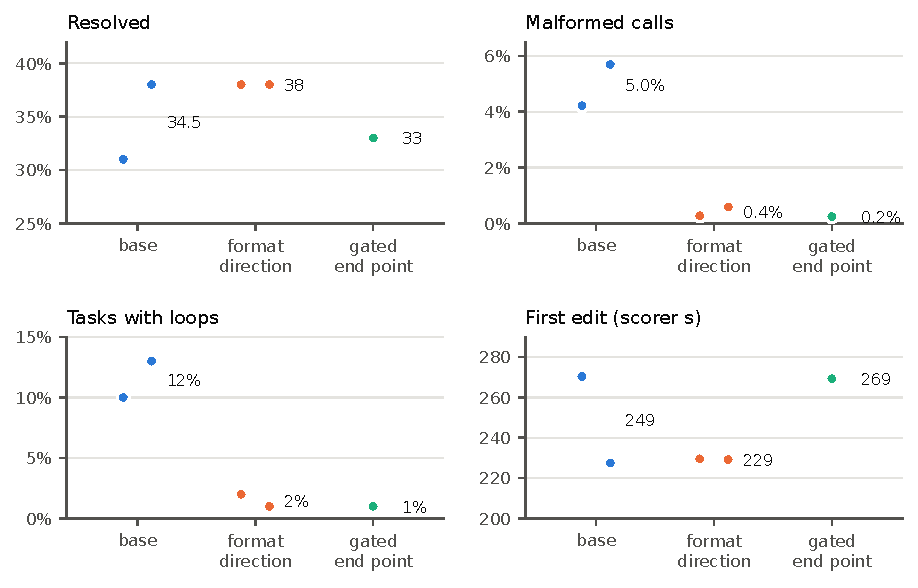
\includegraphics[width=\linewidth]{figures/main_100.pdf}
  \caption{The 100 sound public tasks at the calibrated budget; each dot is one independent draw and each label the mean over draws. Malformed calls and loops separate the arms in every draw; resolution and time to the first edit do not (the base's two draws span the format direction's).}
  \label{fig:main}
\end{figure}

\begin{table}[t]
\centering
\small
\begin{tabular}{lccccc}
\toprule
 & base (1) & base (2) & format (1) & format (2) & gated end \\
\midrule
Resolved / 100 & 31 & 38 & 38 & 38 & 33 \\
Malformed calls & \textbf{4.2\%} & \textbf{5.7\%} & \textbf{0.3\%} & \textbf{0.6\%} & 0.2\% \\
Tasks with loops & \textbf{10\%} & \textbf{13\%} & \textbf{2\%} & \textbf{1\%} & 1\% \\
First edit (scorer s, median) & 270 & 227 & 230 & 229 & 269 \\
Wrong edits & 45\% & 43\% & 39\% & 40\% & 46\% \\
Patches touching source & 76\% & 81\% & 77\% & 78\% & 79\% \\
Compactions per task & 1.04 & 1.01 & 1.03 & 1.08 & 0.96 \\
\bottomrule
\end{tabular}
\caption{Same 100 tasks, same budget, independent draws. Bold: the coordinates on which the two arms separate in every pair of draws. Pooling the two draws per arm and pairing by task, the format direction's resolution is 3.5 points higher (95\% paired-bootstrap interval $-1.5$ to $+8.5$; 13 tasks lean to it and 5 to the base, sign test $p = 0.10$).}
\label{tab:main}
\end{table}

The direction does what it was trained for, and that replicates. Malformed calls fall from 127 and 176 of about 3,000 to 9 and 18, and tasks with exact-repeat loops from 10 and 13 to 2 and 1, in every pairing of a base draw with a format draw, while turn counts, compactions and the edit rate are unchanged.

Whether it raises resolution is a different question, and this comparison is a cautionary tale about answering it. After one base draw (31) and two format draws (38, 38), the gain looked replicated: seven tasks twice, with discordant tasks favouring the direction three to one. A second base draw at identical settings, with the same server throughput and the same number of timeouts, resolved 38, and the apparent earlier first edit (270 against 230 seconds) disappeared with it (227). Pooled, the direction is 3.5 points ahead with an interval that includes zero, and de-biasing for selection (Section~\ref{sec:measure}) leaves the difference unchanged, with a model standard deviation of 2.5 tasks. We read this as: the direction removes a real failure mode at no cost in score, and its score benefit on these public repositories, if any, is smaller than the run-to-run noise of 100 tasks. Replicating only the treatment arm produced a confident and wrong claim, which an earlier draft of this paper made.

\paragraph{Leaderboard.} The bundle with this direction scores 0.13 on the public leaderboard, which runs on private repositories the model has not seen. The public score is a count over 58 tasks truncated to two decimals: 58 is the only task count that reproduces every distinct score on the board, as public analyses also found~\citep{afshar2026draws}. Our 0.13 is therefore 8 tasks, from one draw. The board shows each team's best draw. Among its 4,849 teams on 5 November 2026 the median is 9 tasks, 6 for teams with one submission and 11 for teams with 17 to 40, and the 76 teams at 13 tasks or more (0.22 and above) have a median of 18 submissions. Repeated public submissions of identical files~\citep{afshar2026draws,gluzdov2026evidence} put one draw's standard deviation at 1.6 tasks; the most-run public configuration averages 10.0 of 58 over ten draws, and the files behind one 0.22 badge re-drew 7 to 10 on seven later runs. The entries at 0.22--0.24 are thus consistent with top draws of agents worth about 10 tasks (the leader, at 17, stands three tasks clear), and our distance to the best-documented public agent is two tasks, inside one draw's noise. Section~\ref{sec:gap} locates the gap to our 34.5--38\% on public repositories; a single leaderboard score cannot separate the direction from the base in any case.

\section{Results: query-only control}\label{sec:results-control}

\paragraph{Sampling knobs alone.} A pilot controlled temperature, thinking budget, the prompt's read-window size and the tool-call cap toward a target of fewer malformed calls, loops and empty patches and a faster first edit. Its Jacobian (Table~\ref{tab:cond}) has singular values 3.57, 1.69, 0.45 and 0.006: the tool-call cap has no measurable effect at this budget, and the pseudo-inverse correctly drops it rather than stepping along it. Over four steps the controller drove the three live knobs to their upper bounds (temperature 1.0, thinking 2,048, read window 150) while the whitened residual went 26.7, 17.4, 24.0, 16.0. Re-run twice on dev24, that end point resolved 7 and 8 of 24 against the base's 10 and 9, with malformed calls at 7.5\% and 5.8\%. Single draws on rotating task chunks had hidden the cost on the coordinates the controller was not pushing.

\begin{table}[t]
\centering
\small
\begin{tabularx}{\linewidth}{Lccc}
\toprule
Control set & singular values of $G$ & condition & strongest lever \\
\midrule
Sampling knobs: temperature, thinking budget, read window, tool-call cap & 3.57, 1.69, 0.45, 0.006 & 591 & temperature \\
Directions: format weight, decisiveness weight; plus temperature & 7.21, 2.17, 1.29 & 5.6 & format weight \\
\bottomrule
\end{tabularx}
\caption{Prior Jacobians on the transformed behaviour scale, one forward difference per column on a fixed 24-task batch.}
\label{tab:cond}
\end{table}

\paragraph{Directions as controls.} Over the format and decisiveness weights plus temperature, the Jacobian is well conditioned (Table~\ref{tab:cond}): each direction has a dominant coordinate, and the format weight is the strongest lever in either control set ($-5.3$ logits of malformed-call rate per unit weight). The most useful single observation of the control phase is a compensation (Table~\ref{tab:compensation}): at temperature 1.0, which alone raised malformed calls to 6--8\% and cost resolution, a format weight of 2 holds them at 0.1--0.5\% and resolution at the base's level. This is the mechanism a controller over directions relies on: a knob can be spent on one coordinate while a direction pays for its side effects.

\begin{table}[t]
\centering
\small
\begin{tabularx}{\linewidth}{Lccc}
\toprule
Configuration (dev24, two draws each) & temperature & malformed calls & resolved / 24 \\
\midrule
Base (no direction) & 0.2 & 2.0\%, 2.9\% & 10, 9 \\
Knob controller's end point (no direction; thinking 2,048, read window 150) & 1.0 & 7.5\%, 5.8\% & 7, 8 \\
Direction controller's end point (format 2.0, decisiveness $-0.5$) & 1.0 & 0.1\%, 0.5\% & 10, 9 \\
\bottomrule
\end{tabularx}
\caption{A direction compensates a harmful knob. The two end points differ in more than temperature, so this is an observation about operating points, not a controlled ablation of temperature.}
\label{tab:compensation}
\end{table}

\paragraph{Trajectories.} Figure~\ref{fig:traj} shows the whitened residual along each controller run. Ungated and with targets set beyond what the controls can reach, both the knob controller and the first direction controller ran to their bounds without reducing the residual. With targets moved to where the measured responses say they are attainable, every draw on the fixed dev24 set, and the merit gate, the third run started at a residual of 4.8 and hovered between 3.6 and 9.8 while its moves stayed small and inside the trust region. A second gated run, before the gate's reference was made noise-aware, rejected two re-draws of its own reference point, because a fixed reference with a one-task allowance sits inside the per-draw noise. The gated end point (format 1.14, decisiveness 0.34, temperature 0.34) resolved 10 and 7 of 24 on dev24 and 33 of 100 on the full set, within the range of the other agents' draws (31 to 38), and kept the format behaviour (0.2\% malformed calls).

\begin{figure}[t]
  \centering
  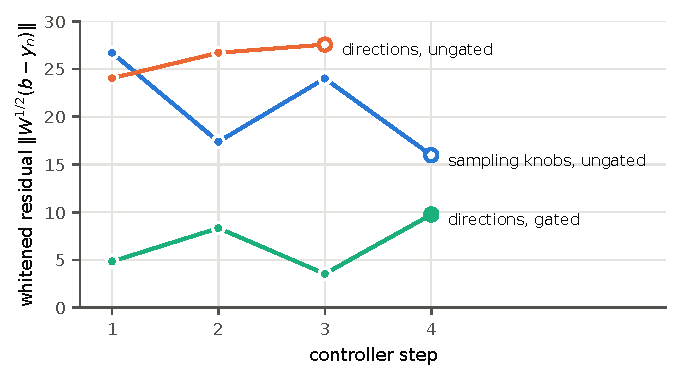
\includegraphics[width=\linewidth]{figures/trajectories.pdf}
  \caption{Whitened residual $\|W^{1/2}(b - y_n)\|$ along each controller run. Hollow markers end at the box bounds. The gated run uses attainable targets and a fixed task set, so its scale is not comparable with the ungated runs'; what differs is that it stays near its starting point instead of running to a bound.}
  \label{fig:traj}
\end{figure}

\paragraph{The decisiveness direction.} Isolated at temperature 0.2 with the format weight fixed at 1, a decisiveness weight of $+1$ raised the edit rate (79\% and 92\% against 71\%) and cut empty patches (13\% and 4\% against 25\%), but raised wrong edits; a weight of $-0.5$ gave the earliest first edit (201 and 195 seconds) and fewer edits. Resolution stayed within noise (8 to 10 of 24) at every weight. The direction is a tilt that trades empty patches against premature edits, and not a source of score on this task distribution.

\section{Where the leaderboard gap comes from}\label{sec:gap}

Locally the unmodified agent resolves 31--38\% of the public tasks; on the leaderboard's hidden private repositories, 13\%. We tested four explanations in turn (Figure~\ref{fig:ladder}).

\paragraph{The scoring environment.} A private notebook on the scoring hardware ran the agent on 30 public tasks under scoring conditions (the official server settings, the five-minute cap, tasks one at a time). It resolved 10, against 8, 12, 11 and 10 in four local draws of the same tasks, and every task it resolved was also resolved locally. The local budget calibration holds, and the environment does not explain the gap. (A gold-patch control in the same notebook passed only 22 of the 30 tasks: the notebook environment lacks a test library that eight \texttt{fastapi} tests import. This affects public tasks run in notebooks, not the hidden-set scoring.)

\paragraph{Repository familiarity.} We mined 2026 commits from less-known, actively maintained, pure-Python repositories (338 to 8.8k GitHub stars) that change package source and tests, and built tasks in the harness's format: the commit's source diff as the gold patch, its test diff as the hidden tests, its message as the problem statement, and the parent tree as the snapshot. Of 120 tasks from 12 repositories, 95 are sound (the gold patch passes and an empty patch fails). The agent resolves 59\% of them, more than the public tasks: unfamiliarity does not lower its score.

\paragraph{Fix size.} From 18 repositories we built 106 tasks with larger fixes (at least 40 changed source lines or at least two source files; median 47.5 lines over two files, against 16 for the first set), 76 of them sound. The agent resolves 37\%, the public level. Its first edit comes at a median 261 of the 300 scorer-seconds, so larger fixes squeeze the budget, but they do not reproduce the leaderboard's level.

\paragraph{Problem-statement informativeness.} The same 76 tasks with each statement cut to its pull-request title (``fix: accept tuples for list-valued options'') drop to 17\%: 15 tasks lost and none gained against the full commit messages, exact sign test $p = 0.0001$. Wrong edits rise from 51\% to 62\% and empty patches double. Of the 15 lost tasks, about six changed only part of what the fix needed (a synchronous code path but not its asynchronous twin, an implementation but not the package export of a new function, one of the four modules that read an option), seven timed out, and the rest edited the right files with the wrong semantics. The effect replicates on the public tasks: cut to their titles, the 100 sound tasks drop from 31 and 38 resolved (two draws with the full pull-request text) to 21 (16 lost and 6 gained against the first draw, $p = 0.05$; 21 lost and 4 gained against the second, $p = 0.0009$). Empty patches rise to 33\% from 17\% and 12\%, and the median first edit slips to 294 of the 300 scorer-seconds: with a title alone the agent more often never settles on what to change. Public statements are pull-request titles with descriptions; we infer that the hidden statements carry about as little information as a title, which accounts for most of the gap.

\paragraph{How much of a statement is a hidden task worth?} We made that inference a measurement with the one-dimensional form of the iE iteration of Section~\ref{sec:control}. The knob is the fraction $f$ of each statement's body kept after the title (the first $\lceil fL \rceil$ of its $L$ non-empty lines), $M(f)$ is the agent's resolution rate on the 76 hard tasks, and $\alpha$ is the leaderboard's 0.13 (8 of 58 tasks, 0.138; the iteration ends the same way at either value). From a first draw at $f = 0.5$ (21 of 76) the Newton step with the secant gain of the two end points asked for $f = -0.24$, clipped to the title-only bound, where a replicate draw gave 13 again and the residual kept its sign: the equation has no root in $[0, 1]$. Title-only is the nearest point and lies 3.3 points above the leaderboard's 8 of 58, 0.6 standard errors of the difference, so on this set the hidden statements are worth at most a title and the remainder of the gap is inside the noise. A curve point at $f = 0.25$ (15 of 76) shows the information is not front-loaded: the first quarter of the body adds two tasks, the second quarter six and the second half seven. The replicate also gives the proxy its noise floor: the two title-only draws share 10 resolved tasks and swap 3 each way, so the agent variants at 13 of 76 in Section~\ref{sec:scaffold} are indistinguishable from re-draws of the base.

\paragraph{A smaller, faster model.} The 12B model is twice as fast as the 31B on the scoring hardware (67--78 against 35--39 decode tokens/s), so it gets about twice the turns in five minutes. It is worse: 6 against 10 of the 30 public tasks on the scoring hardware (19 against 12 timeouts, a median 53 tool calls against 27), and 40\% against 59\% on the first held-out set. It spends the extra turns without converging.

\begin{figure}[t]
  \centering
  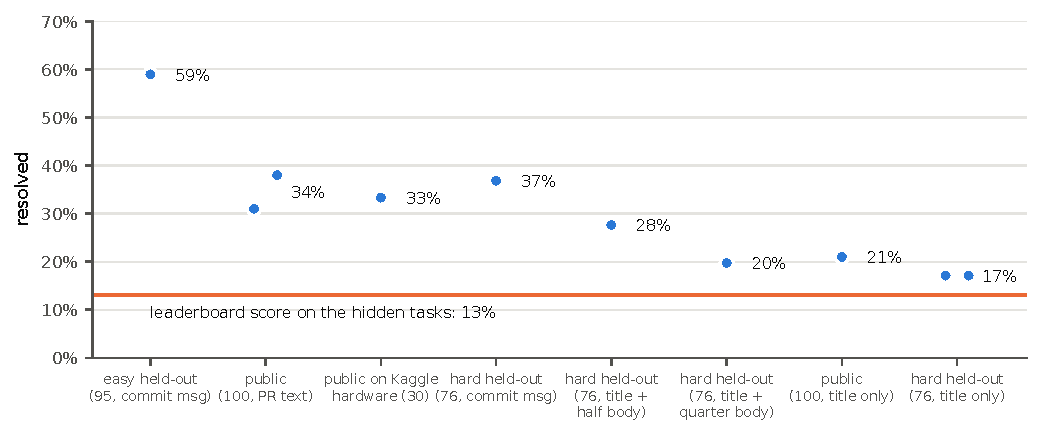
\includegraphics[width=\linewidth]{figures/difficulty_ladder.pdf}
  \caption{The unmodified 31B agent's resolution rate on each task set at the calibrated budget (one dot per independent draw), against its leaderboard score on the hidden tasks. Only cutting statements to a title brings a local set near the leaderboard, on both the public and the hard held-out tasks; keeping a quarter or a half of the statement body moves the hard set between its two ends.}
  \label{fig:ladder}
\end{figure}

\section{Scaffold and adapter changes on a leaderboard-matched proxy}\label{sec:scaffold}

The title-only set is the closest local match to the leaderboard, so we used it to test five changes aimed at the failures above (Table~\ref{tab:scaffold}).

\begin{enumerate}
  \item \textbf{Code-search and test tools.} An ADK skill with two scripts the agent runs in its sandbox: one ranks the source files for identifiers from the statement and shows the enclosing functions and related test files in about 60 lines; the other finds the tests related to the agent's edits, runs them with a time limit and prints only the summary and the first failure.
  \item \textbf{Speed.} Thinking off, which roughly halves the time per turn, with the format direction to keep the calls well formed.
  \item \textbf{Guidance for terse titles.} The tools plus a prompt section on what a title usually implies: read the existing tests of the code first; make the change everywhere it applies (synchronous and asynchronous variants, sibling functions, every reader of a changed option); export new names where their siblings are exported.
  \item \textbf{Statement distillation.} A direction that teaches the agent to act from a title as it would from the full statement, trained with a privileged teacher~\citep{chen2020cheating} at the student's own states, as in DAgger~\citep{ross2011dagger}. We ran the base agent title-only on the public tasks; at each of its first eight steps on the 40 tasks the informed agent had solved, the same model sampled the next call twice from the student's context and twice from that context with the full statement in place of the title. Where a teacher call differed materially from a student call (another kind of action, or files and search terms that overlap by less than half), the pair keeps the student's own thought on both sides, with the teacher's call as chosen and the student's as rejected, so the statement never enters the training text. This gave 307 pairs at 156 states over 39 tasks from the two public repositories. The direction was trained as before (rank 16, NLL-anchored DPO, prompts up to 8,192 tokens), stopped early after 80 states, and was evaluated at weight 1 on the held-out repositories, none of which it saw in training.
  \item \textbf{Imitation of whole informed trajectories.} The same goal by supervised fine-tuning: 153 trajectories in which the agent with the full statement resolved its task (the public tasks and the easier held-out set, minus the eight tasks shared with the evaluation set), rendered with the statement cut to its title, and the model trained to emit the informed agent's thought and call at each of 1,530 steps. A thought that quotes the statement is kept as context but masked from the loss. The steps of a trajectory share one key-value cache, which is exact because Gemma~4 keeps calls and responses inside one model turn, so each step's prompt extends the previous one; prompts were capped at 8,192 tokens, with later edits trained on a truncated context.
\end{enumerate}

\begin{table}[t]
\centering
\small
\begin{tabularx}{\linewidth}{Lccccc}
\toprule
Agent (76 title-only tasks) & resolved & lost / gained & wrong edits & empty patches & loops \\
\midrule
Base (thinking 512) & 13 & -- & 62\% & 20\% & 14\% \\
+ code-search and test tools & 13 & 3 / 3 & 59\% & 20\% & 9\% \\
Thinking off + format direction & 4 & 10 / 1 & 58\% & 34\% & 41\% \\
+ tools + guidance for terse titles & 13 & 3 / 3 & 51\% & 30\% & 8\% \\
Statement-distilled direction & 13 & 4 / 4 & 61\% & 20\% & 8\% \\
Imitation of informed trajectories & 13 & 3 / 3 & 62\% & 18\% & 8\% \\
\bottomrule
\end{tabularx}
\caption{Scaffold and adapter changes on the leaderboard-matched proxy; ``lost / gained'' counts tasks against the base, paired by task.}
\label{tab:scaffold}
\end{table}

The tools were used heavily (the search script in 66 of 76 tasks, the test script in 41) and reduced malformed calls and loops, but they also added context compactions (1.42 against 1.01 per task) and delayed the first edit; the score did not move. The guidance did what it asked for, lowering wrong edits from 62\% to 51\%, and a more careful agent ran out of time before editing more often; the score did not move. Without thinking the agent reached its first edit in 147 instead of 241 scorer-seconds and took twice the turns, but looped in 41\% of the tasks and resolved two thirds fewer. The distilled direction halved malformed calls (2.3\% against 4.7\%) and loops, and moved the first edit later (302 against 241 scorer-seconds), but traded four tasks for four others. Its pairs were weak: two student samples at the same state differ materially in 25\% of cases and two teacher samples in 30\%, against 41\% for a student and a teacher sample, so only about a third of the pairs carry what the statement adds. Every change shifted behaviour and traded tasks rather than adding them.

\paragraph{How much of a pair set is signal, and how to raise it.} The statement miner emits a pair where one student sample and one teacher sample differ materially, and sampling noise makes two samples from the same side differ too. Its criterion has one continuous knob, a Jaccard cutoff $t$ on the calls' targets, so the false-pair rate can be set by the stationary equation $M(t) = \alpha$ with $M$ the same-side disagreement rate. At 168 fixed title-only states from unseen repositories, with four samples per side, $M$ is observed directly and the equation is solved by monotone search, with a split-half check. The curve is a staircase: the same-side rate is 5\% with no target comparison, jumps to 15\% as soon as disjoint targets count, and is 20\% at the cutoff we used, where the cross-side rate is 33\% and 37\% of emitted pairs are signal. A 5\% false-pair rate is reached only by ignoring targets, where the cross-side rate is 6\%: the statement's effect is in where the agent looks, and no cutoff separates it from the student's own stochasticity at these states. Consensus does: emit a pair only where two samples on each side agree and the two sides' consensus decisions differ. Measured on disjoint halves of the samples, that gives a false-pair rate of 2--4\%, 78--83\% of pairs signal, and 10--11 pairs per 100 states, the same number of signal pairs as single-sample mining at four times the purity, for four samples per side instead of one. The same data put a number on what the title lacks: under the mixture ``either the statement matters at this state or cross-side disagreement is same-side noise'', the statement changes the agent's next call at 12--15\% of early states, about one in seven. We did not retrain on consensus pairs: the distilled direction's failure, below, is the absence of the information, not the purity of the pairs.

\paragraph{Calibrating the distilled direction with iE.} With two thirds of its pairs noise, the distilled direction could be a shrunk estimate of the teacher's shift, which is the setting iE was built for: find the parameter whose simulated statistic matches the observed one, $M(w^*) = \alpha$~\citep[Section~3.3]{qin2025ie}. We used 168 title-only states of the base agent on the 28 hard held-out tasks that the informed agent solved, from repositories absent from the training pairs. The observed $\alpha$ is the probability that two independent teacher samples agree (are not materially different); the simulated $M(w)$ is the probability that a sample of the title-only agent with the direction at weight $w$ agrees with a teacher sample. If the agent's next call had the teacher's distribution, $M(w) = \alpha$ exactly; a malformed sample counts as disagreement on both sides. One draw of $M$ at fixed states takes about 15 minutes, against 4.5 hours for an agent run on the 76 tasks. The equation has no root (Figure~\ref{fig:iemoment}). $M$ is highest near the base (0.68 at $w = 0$, 0.69 at $w = -1$), falls to 0.64 at the trained weight (paired difference $-0.041$, standard error 0.020), and collapses below $w = -1$ as calls stop parsing, while $\alpha = 0.78$. With a negative gain the iteration stepped to the lower bound, where a guard on malformed calls rejected every draw. On unseen repositories the direction moves the agent's next call away from the informed teacher's, and no weight brings it closer than the base: what separates the title-only agent from the informed one is information the title lacks, not a bias in the policy that a weight could remove.

\begin{figure}[t]
  \centering
  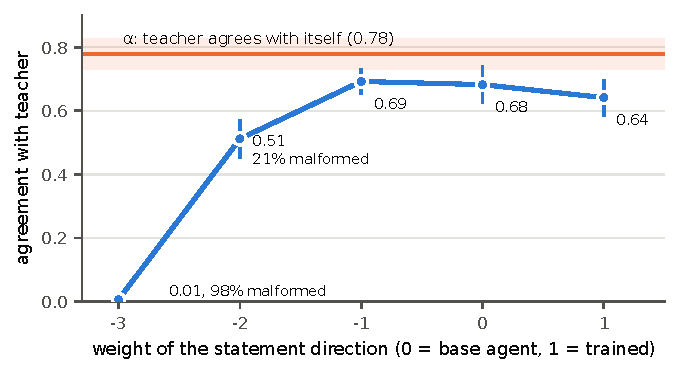
\includegraphics[width=0.72\linewidth]{figures/ie_moment.pdf}
  \caption{iE calibration of the statement direction at 168 title-only agent states from repositories it was not trained on. Each point is the mean agreement of the agent's next call with a full-statement teacher's (bars: 95\% intervals; $w = -1$ pools two draws and $w = -3$ four); the band is the teacher's agreement with itself, the value the iteration seeks. No weight reaches it, and the trained weight ($w = 1$) is further from it than the base.}
  \label{fig:iemoment}
\end{figure}

\paragraph{How far a fixed-state check generalises.} These draws sampled at temperature 0.6 with unbounded thoughts, because the server's raw completion endpoint ignores the thinking budget that its chat endpoint enforces. With the agent's own sampling (chat endpoint, temperature 0.2, 512-token thinking budget, the harness's tool-call parser) the result holds: at 84 teacher states agreement falls from 0.82 at $w = 0$ to 0.78 at $w = 1$ and 0.68 at $w = 2$, against $\alpha = 0.86$. We then asked whether the same check could gate any new direction before an agent run, and tested it against the agent runs we already had. At 300 states of the public tasks (three per trajectory, before any context compaction) and 224 of the hard set, it measured each direction's change in malformed calls, exact repeats of the previous call, edits and tokens per call, paired by state. It did not predict the agent-level changes. The format direction cut malformed calls from 5.0\% to 0.4\% and loops from 11.5\% to 1.5\% in agent runs; at fixed states it moved malformed calls by $-0.8$ points (standard error 0.5) and repeats by $+0.9$ (0.8), so a gate would have rejected the one direction that worked. The decisiveness direction raised edit attempts from 75\% to 88\%; at fixed states its edit share moved by $+0.8$ points (0.6). Of 20 comparisons one fixed-state change was distinguishable from noise, and it had the opposite sign to the agent's. These effects act through the trajectory: a direction that avoids a failure state, or nudges each call slightly towards an edit, changes which states the agent reaches, which single calls at the base agent's states cannot show. The fixed-state check is a sound gate for per-call objectives such as agreement with a teacher, and not for loops, malformed calls or edit timing.

\paragraph{Imitating whole trajectories.} The trajectory-imitation adapter is the cleanest title-only agent we have: malformed calls 1.1\% against the base's 4.7\%, loops 8\% against 14\%, fewer scratch files, slightly more edits, and the same first-edit time. It resolves 13 tasks, three lost and three gained. Its training loss explains why. Before any training, the base model already assigned the informed agent's calls a mean 0.07 nats per token in title-only context: at most steps the informed agent does what the title-only agent would do anyway. The statement decides a few steps, such as which file to change or whether the fix has a second half, and imitating the rest does not supply what those steps need.


\paragraph{iE as the outer loop of DPO.} The controllers of Section~\ref{sec:results-control} steered the merge weights of fixed adapters. A stronger form of the same question puts iE outside the training itself: each draw retrains one adapter from scratch at training settings $x$ (the primal step), evaluates it, and iE moves the settings (the dual step), in the single-draw Robbins--Monro form. The knobs were the loss weights of the format and hindsight pair sources and the early-stop margin, all on the log scale. Each draw retrained on a fixed seeded 120 pairs (about two hours), merged the adapter into the agent and ran a fixed 24-task batch of the title-only hard set (1.5 hours). Targets were ceilings on malformed calls (1\%), loops (3\%), the first edit (200 scorer-seconds), empty patches (12\%) and compactions (1.0), whitened by three base-like runs on the batch with a floor per coordinate, and the merit gate protected resolution with a two-task allowance; a retrain the trainer's gates refuse counts as an infeasible point and rejects the move without an evaluation. Table~\ref{tab:ietrain} gives the eight draws. Mechanically the loop worked: no retrain was refused, every draw passed the gate, and the probed Jacobian has condition 11.4 and localises each knob (the stop margin is the malformed-call knob; halving the decisiveness weight brings loops back and cost three resolved tasks, the first resolution effect that source has shown). As a controller it reduced nothing: the residual was 3.2 at the probe base and 4.9, 5.5, 4.3 and 4.0 over the four steps. The retrain at the anchored settings already satisfied the three format-side ceilings, so the residual was the first edit and empty patches, and neither responded to the knobs at the resolution of one draw. Across the eight retrains the first edit's spread (0.12 in log units) equals the noise runs', and its correlation with the log format weight is $-0.56$, the opposite sign to the Jacobian entry that a single probe draw had set, so the fixed-Jacobian iteration walked the format weight from 1.0 to 0.14 on the strength of one low draw. The pairs reach the format coordinates, which a fresh adapter already satisfies, and not the planning coordinates that decide resolution on this set, so the outer loop has nothing to steer: the directions controller's null, reached through the training settings instead of the merge weights. Two method notes. With equality targets, as iE is stated, the first step would have spent itself raising malformed calls and loops back to targets the retrain had overshot, which is why the targets are ceilings (the residual is clipped at zero on the satisfied side). And a Jacobian column should come from more than one draw when a coordinate's draw-to-draw spread is comparable to its response.

\begin{table}[t]
\centering\footnotesize
\caption{iE as the outer loop of DPO on a fixed 24-task batch of the title-only hard set. $x$ is (format weight, decisiveness weight, stop margin); the residual is the whitened one-sided distance to the targets. Three base-like runs on the batch: malformed 0.7--2.3\%, loops 8--13\%, first edit 276--301 s, empty 17--29\%, resolved 3, 4, 4.}
\label{tab:ietrain}
\setlength{\tabcolsep}{3.5pt}
\begin{tabular}{llrrrrrrr}
\toprule
draw & $x$ & malformed & loops & first edit & empty & compact. & resolved & residual \\
\midrule
probe, base & 1.00, 1.00, 1.5 & 0.4\% & 0\% & 274 s & 25\% & 0.88 & 5 & 3.2 \\
probe, format halved & 0.50, 1.00, 1.5 & 0.3\% & 0\% & 240 s & 21\% & 1.17 & 5 & 2.3 \\
probe, decisiveness halved & 1.00, 0.50, 1.5 & 0.5\% & 8\% & 265 s & 29\% & 1.21 & 2 & 4.8 \\
probe, margin 2.4 & 1.00, 1.00, 2.4 & 0.0\% & 4\% & 275 s & 21\% & 1.38 & 5 & 3.5 \\
step 1 & 0.61, 0.96, 1.2 & 0.0\% & 8\% & 325 s & 21\% & 1.17 & 4 & 4.9 \\
step 2 & 0.37, 1.20, 0.9 & 0.1\% & 8\% & 338 s & 25\% & 1.33 & 4 & 5.5 \\
step 3 & 0.22, 1.45, 0.8 & 0.3\% & 0\% & 316 s & 29\% & 1.08 & 4 & 4.3 \\
step 4 & 0.14, 1.42, 0.8 & 0.3\% & 0\% & 318 s & 25\% & 1.00 & 4 & 4.0 \\
\bottomrule
\end{tabular}
\end{table}

\paragraph{The informed agent's behaviour as the target.} The controllers above aimed at targets we set. A last run asks the equation a sharper question: is the behaviour of the agent that sees the full statements (28 of 76 on the hard set) a point the title-only agent's controls can reach? Its measured behaviour vector is the target, as equalities on the source-edit, wrong-edit and empty-patch rates and ceilings on the first edit, malformed calls and loops; the controls are the merge weights of the decisiveness, trajectory-imitation and statement-distillation directions and the log thinking budget; every draw is the full 76-task title-only set, so each Jacobian column is a 76-task difference, and the Jacobian is re-estimated by a ridge fit over all draws after every step. The base and two columns came from existing draws and two columns were drawn (Table~\ref{tab:informed}). The probe Jacobian has singular values 3.9, 0.6, 0.2 and 0.1: its one strong direction is the three adapters acting together on malformed calls and loops, where they are nearly collinear, and the edit coordinates, where the target differs from the base, lie on the weak ones. Projected on the Jacobian's span, 54\% of the squared whitened residual at the base is unreachable to first order with all four columns, and 77\% at the rank the gain keeps. The first move cut the thinking budget to 311, the one column whose edit entries pointed the right way together; the draw moved the opposite way on both edit coordinates. The refit over seven draws cut that column's edit entries to a sixth and dropped the second singular value below the rank cutoff, so after one more step, computed before the refit, the controller stood still; step 3 is a re-draw of step 2's point and shows the proxy's noise there (12 and 11 resolved, loops 26\% and 20\%). The residual went 4.5, 6.2, 7.0 and 5.3 and never fell below the base's, while the merit gate accepted every step: 13, 12 and 11 resolved against an allowance of 4.5 tasks, a drift the gate cannot tell from noise. The target was unreachable by construction: source edits equal resolution plus wrong edits in every draw, so its edit coordinates ask for 28 of 76 by another name. Over seven title-only draws the agent resolved 20 distinct tasks, 17 of them among the informed agent's 28; 11 of the informed agent's tasks were never resolved from a title. Re-estimating the Jacobian did what the fixed-gain runs lacked: it caught a wrong sign after one step instead of following it to a bound.

\begin{table}[t]
\centering\footnotesize
\caption{The informed agent's behaviour as the target, on the 76-task title-only hard set. $x$ is (decisiveness, trajectory and statement weight; thinking budget); the residual is the whitened one-sided distance to the full-statement base draw's behaviour (28 resolved). The trajectory and statement columns are the weight-1 draws of Section~\ref{sec:scaffold}.}
\label{tab:informed}
\setlength{\tabcolsep}{3.5pt}
\begin{tabular}{llrrrrrrr}
\toprule
draw & $x$ & source & wrong & empty & loops & malf. & resolved & residual \\
 & & edits (\%) & edits (\%) & (\%) & (\%) & (\%) & / 76 & \\
\midrule
base, two draws & $0, 0, 0$; 512 & 79, 74 & 62, 57 & 20, 22 & 14, 13 & 4.7, 5.9 & 13, 13 & 4.1, 5.1 \\
probe, decisiveness & $1, 0, 0$; 512 & 80 & 62 & 18 & 2.6 & 0.3 & 14 & 3.8 \\
probe, trajectory & $0, 1, 0$; 512 & 79 & 62 & 18 & 7.9 & 1.1 & 13 & 3.9 \\
probe, statement & $0, 0, 1$; 512 & 78 & 61 & 20 & 7.9 & 2.3 & 13 & 4.3 \\
probe, thinking & $0, 0, 0$; 1024 & 72 & 55 & 25 & 13 & 6.8 & 13 & 6.0 \\
step 1 & $-0.14, 0.32, -0.22$; 311 & 70 & 53 & 29 & 10 & 3.4 & 13 & 6.2 \\
step 2 & $-0.45, 0.82, -0.64$; 189 & 66 & 50 & 28 & 26 & 4.3 & 12 & 7.0 \\
step 3 & $-0.41, 0.84, -0.63$; 188 & 74 & 59 & 22 & 20 & 5.3 & 11 & 5.3 \\
target & & 88 & 51 & 11 & $\le 13$ & $\le 4.6$ & 28 & 0 \\
\bottomrule
\end{tabular}
\end{table}

Together with the earlier prompt and sampling sweeps, the format direction and the controllers, this is a consistent picture: on underspecified tasks under a five-minute budget, the model's own reasoning is the binding constraint.

\section{Lessons}\label{sec:lessons}

\begin{itemize}
  \item \textbf{Calibrate the budget before believing a comparison.} Our early conclusion that the thinking-on agent ``cannot reach an edit'' was an artifact of running at a third of the real budget.
  \item \textbf{Steer by behaviour, decide by paired score at scale.} Behaviour coordinates separate configurations in one 24-task draw; resolution differences of a few points need 100 tasks and repeated draws.
  \item \textbf{Redraw the control, not only the treatment.} Two draws of the base agent on the same 100 tasks, at identical settings and with indistinguishable infrastructure, resolved 31 and 38. Our replicated seven-point gain was the low base draw.
  \item \textbf{Check a direction by generating with it, with a check sized to the mode.} DPO training metrics were perfect for an adapter that was unusable; a one-minute greedy generation would have caught it. The same check, with a 256-token cap set for thinking off, later rejected a sound thinking-on adapter whose call wrote a short script.
  \item \textbf{On-policy contrast is not always available.} Where the model is already right (just before a successful edit) or almost never right (early in a trajectory), hindsight pairs supply the chosen side.
  \item \textbf{A query-only controller needs a gate, a reachable target and a Jacobian it can trust.} Without the first two it does what stochastic approximation is designed to do, pursue the largest residual, straight into a bound. An equality target a point already beats pushes it back; targets should be ceilings. A column probed from one draw, on a coordinate whose draw-to-draw spread matches its response, can carry the wrong sign, and the fixed-gain iteration follows it for the rest of the run; re-estimating the Jacobian from every draw caught such a sign after one step. A target taken from another agent's measured behaviour can be unreachable by construction, because edit rates are identities of the score.
  \item \textbf{Build a local set that matches the leaderboard before tuning against it.} Our public, unfamiliar-repository and large-fix sets all overstated the hidden-set score by two to four times; only shortening the statements reproduced it. A scaffold change that looks neutral on an easy set could still matter on the hard one, and vice versa.
  \item \textbf{Check per-call targets at fixed states, trajectory-level ones in agent runs.} A moment equation at fixed agent states costs a fraction of an agent run and showed that the distilled direction moves the agent away from its teacher, which the 4.5-hour agent run confirmed. The same check, validated against our other directions, missed the format direction's effect on malformed calls and loops, which acts through the trajectory, and would have rejected the one direction that worked.
  \item \textbf{Measure how much of a pair set is signal.} Comparing two samples from the same side gives the noise floor of a disagreement-based miner; for statement distillation it was two thirds of the pairs, and no threshold on the criterion lowers it, while a two-sample consensus per side cuts it to a few percent at no loss of signal pairs.
  \item \textbf{Faster is not better if the model needs its thinking.} Both a twice-as-fast model and thinking off lost to the slower configuration on hard, underspecified tasks.
  \item \textbf{Guard the evaluator.} Two unguarded failures (server starvation and a sandbox out-of-memory kill) each cost a night and would have silently biased results.
\end{itemize}

\section{Related work}\label{sec:related}

Repository-level benchmarks~\citep{jimenez2024swebench} and agent scaffolds~\citep{yang2024sweagent,xia2024agentless} established the setting; training open models for it with trajectories and verifiers is studied in~\citep{pan2024swegym}. We use DPO~\citep{rafailov2023dpo} with an NLL term as in iterative reasoning preference optimization~\citep{pang2024irpo}; failure modes of DPO on pairs with small edit distance are analysed in~\citep{pal2024smaug,razin2024displacement}, and stepwise preference pairs at intermediate states in~\citep{lai2024stepdpo}. Supervising a student at its own states~\citep{ross2011dagger} by a teacher that sees privileged information~\citep{chen2020cheating} is the template for our statement distillation; here teacher and student are the same model with and without the full statement. Low-rank adaptation~\citep{hu2022lora} and arithmetic on task vectors and adapters~\citep{ilharco2023taskarithmetic,huang2023lorahub} motivate treating trained adapters as a basis; our merge is exact for LoRA. iE~\citep{qin2025ie} combines bootstrap iteration~\citep{martin1992double} with stochastic approximation~\citep{robbins1951sa,blum1954approximation}; we use it as a black-box controller rather than for bias reduction.

\section{Limitations}\label{sec:limitations}

The public tasks come from two repositories the model may have seen; the held-out sets add 18 less-known ones, but their tasks are recent commits whose statements are commit messages, not issue reports, and their snapshots carry no git history. Our inference about the hidden statements is indirect: we know only that cutting our statements to a title reproduces the leaderboard's level, not what the hidden statements say. Repositories in the held-out sets were limited to flat-layout pure-Python packages that the local sandbox can import, and some tasks of the easy and hard sets overlap. Our leaderboard result is one draw on 58 tasks, and every local result is conditional on the five-minute frame except where stated. Each configuration has at most two draws on 100 tasks, which is not enough to resolve a difference of a few points: the format direction's pooled advantage of 3.5 points is not distinguishable from zero. The selection-bias correction rests on a two-way model without task-by-configuration interactions, and where the observed spread is below the model's it reports equal rates rather than a root. That the informed agent's behaviour is unreachable is a first-order statement from a four-column Jacobian estimated on nine 76-task draws; a richer control set could span more of it. The behaviour vector and the malformed-call detector are ours, and other definitions would weight the coordinates differently. Training detaches the prefix and, within a completion, earlier chunks; on a tiny random model the chunked gradient has cosine 0.92 with the exact one at a 4-token chunk, which we did not measure at scale. The format and decisiveness directions were trained on prefixes truncated to 4,096 tokens, so they never saw the full contexts at which most malformed calls occur. The statement direction was trained on two public repositories, on half its pairs (early stopping), and evaluated in one draw; a teacher that differs from the student in one step's action cannot convey a multi-step plan. The trajectory imitation used steps before the first context compaction, prompts of at most 8,192 tokens, one epoch, and one evaluation draw; eleven of the easier held-out set's twelve repositories also appear, at other commits, in the evaluation set. The iE calibration measures agreement at the base agent's states, not at the states an adapted agent would reach, with an agreement criterion of our own; the validation of fixed-state checks rests on four direction changes, two of them measured on only 24 tasks. The controller results rest on few steps per run, and the outer loop over DPO on one draw per point, a Jacobian from single forward differences, and a stop-margin knob that proved a staircase (the trainer checks the margin every four steps, so every margin between 0.6 and 1.6 stops at the same step); we make no convergence claim beyond the iE theory, whose monotonicity conditions an agent's behaviour map need not satisfy.

\section{Conclusion}

A rank-16 direction trained on a quantized Gemma~4 agent's own failure states removes most of its malformed tool calls and repeat loops, robustly and at no cost in score; whether that buys score is below what 100 tasks and two draws can resolve. Query-only control with iE over trained directions works mechanically and is well conditioned, and a direction can pay for a knob's side effects, but the controller did not find a better operating point than the single direction. Making the informed agent's measured behaviour the target shows why: more than half of the distance lies outside the directions' span, and the edit coordinates that remain are the score by another name. Placing iE outside the training, as the dual update of DPO's pair weights and stop margin, is feasible and well conditioned and steers nothing either: the pairs reach the format coordinates, which a fresh adapter already satisfies, and not the planning ones. The gap between local and leaderboard scores is mostly the information in the problem statement: cutting statements to a title reproduces the leaderboard's level, and on that proxy neither better tools, nor guidance, nor speed adds score. Under a five-minute budget the limit is the model's reasoning about an underspecified task. Two attempts to train the model to act from a title as it does from a full statement, a direction distilled from a privileged teacher at the agent's own states and imitation of 153 whole informed trajectories, each changed its behaviour on unseen repositories but not its score, and an iE calibration found no weight at which the agent's next call is closer to the informed teacher's than the base model's. The informed agent's calls are already likely under the title-only policy; what the title lacks decides a few steps, and no training on the agent's own behaviour supplies it.

\paragraph{Reproducibility.} Every number above comes from a run folder whose traces, patches and test outputs are kept, and is recorded with its configuration in the project's implementation notes; the miners, trainer, merge, controller and guarded evaluator are single-file scripts.

\bibliographystyle{plainnat}
\bibliography{refs}

\appendix

\section{Rendering the harness context exactly}\label{app:rendering}

The server's tokenization of a rebuilt context and the tokenizer's chat-template rendering agree token for token only if (i) assistant tool-call arguments are passed as objects, not JSON strings (the server parses them before templating, and the template then emits the native bare-key form), and (ii) the system content is a list of text parts (the template's branch for lists appends a space before the first tool declaration). After a call, the model stops by emitting the tool-response opening token, not the end-of-turn token; training targets append it so the adapter learns to stop where the served model does.

\section{Training memory}\label{app:training}

At a 2k-token prefix, two completion graphs of about 480 tokens each held 42\,GiB of activations, because attention scores are materialized on this GPU (about 30\,MB per completion token over 60 layers), and Gemma~4's gradient checkpointing drops a supplied cache. Since the DPO gradient is $\sigma(-m)\,\beta\,(\nabla \log\pi_\theta(y_w) - \nabla\log\pi_\theta(y_l))$, we compute the margin $m$ without gradient, then back-propagate $\mp\sigma(-m)\beta\log\pi_\theta(y)$ for each completion separately and in 96-token chunks. Between chunks the cache is detached, so earlier completion tokens act as constants for later ones. Sliding-window cache layers cannot be cropped once past their window, so the prefix cache is restored for each completion by re-pointing each layer's tensors to a snapshot.

\end{document}
